\documentclass{beamer}
\usepackage[utf8]{inputenc}
\usetheme{Boadilla}
\usecolortheme{seahorse}
\usepackage[french]{babel}
%\usepackage{kpfonts}
\usepackage{tikz}

\usepackage{amsmath} % load the AMS math package
\usefonttheme{professionalfonts} % use the same font for math as in regular LaTeX document
\usepackage{unicode-math} % load a Unicode math font package
%\setmathfont{Latin Modern Math}



\title[Proposition détaillée]{La modélisation de congestion portuaire à l'aide de GNN}
\subtitle{Proposition détaillée}
\author[INF11]{Chef de groupe INF11: Isai Gordeev X22\\}
\institute[]{École Polytechnique\\ Palaiseau}
\date{\today}

\AtBeginSection[]
{
	\begin{frame}
		\frametitle{Outline}
		\tableofcontents[currentsection]
	\end{frame}
}

\AtBeginSubsection[]
{
	\begin{frame}
		\frametitle{Outline}
		\tableofcontents[currentsection,currentsubsection]
	\end{frame}
}

\begin{document}
	
	\begin{frame}
		\titlepage
	\end{frame}
	
	\begin{frame}
		\frametitle{Plan}
			\tableofcontents
	\end{frame}


	\section{Les enjeux et la motivation du travail proposé}
	
	
\begin{frame}
	\frametitle{Les enjeux et la motivation du travail proposé}
	\begin{center}
	Le but d'une grande entreprise logistique est de pouvoir prédire l'état des routes. 
	\end{center}
	
\end{frame}

\begin{frame}
	\frametitle{Les complexités}
	\begin{center}
		\begin{itemize}
			\item Le nombre de ports $N$ est grand pour simuler l'ensemble avec M caractérisations. (Problème à $N\cdot M$-corps )
			\item Les mis à jours deviennent très difficiles
		\end{itemize}
	\end{center}
	
\end{frame}


\begin{frame}
	\frametitle{But plus précisément?}
	Utiliser le GNN temporel pour résoudre les problèmes de la taille et l'évolution du réseau portuaire et surtout pour calculer:
	\begin{itemize}
		\item Le temps d'attente d'un navire
		\item Le nombre de navires en attente
	\end{itemize}
	à partir de données AIS. 
	
	\begin{figure}
	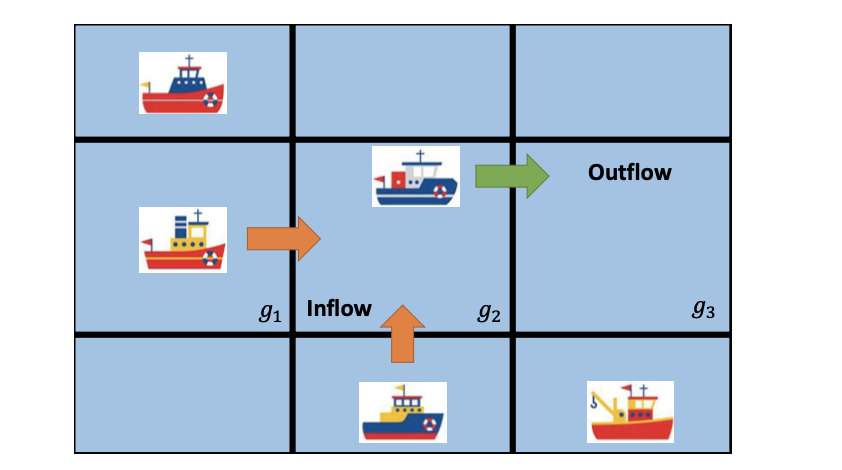
\includegraphics[width=0.8\textwidth]{0}
	\label{fig:example}
	\end{figure}
	
\end{frame}




	\section{La revue et une analyse de l’état de l’art ainsi que des approches concurrentes et alternatives}
	

\subsection{Les approches alternatives}

\begin{frame}
	\frametitle{Les approches alternatives}
	\begin{itemize}
		\item Solution basée sur CNN
		\item Solution basée sur LTSM
		\item Solution hybride basée sur tous les deux
	\end{itemize}

		\begin{columns}[c]
		\column{.3\textwidth}
		\centering
		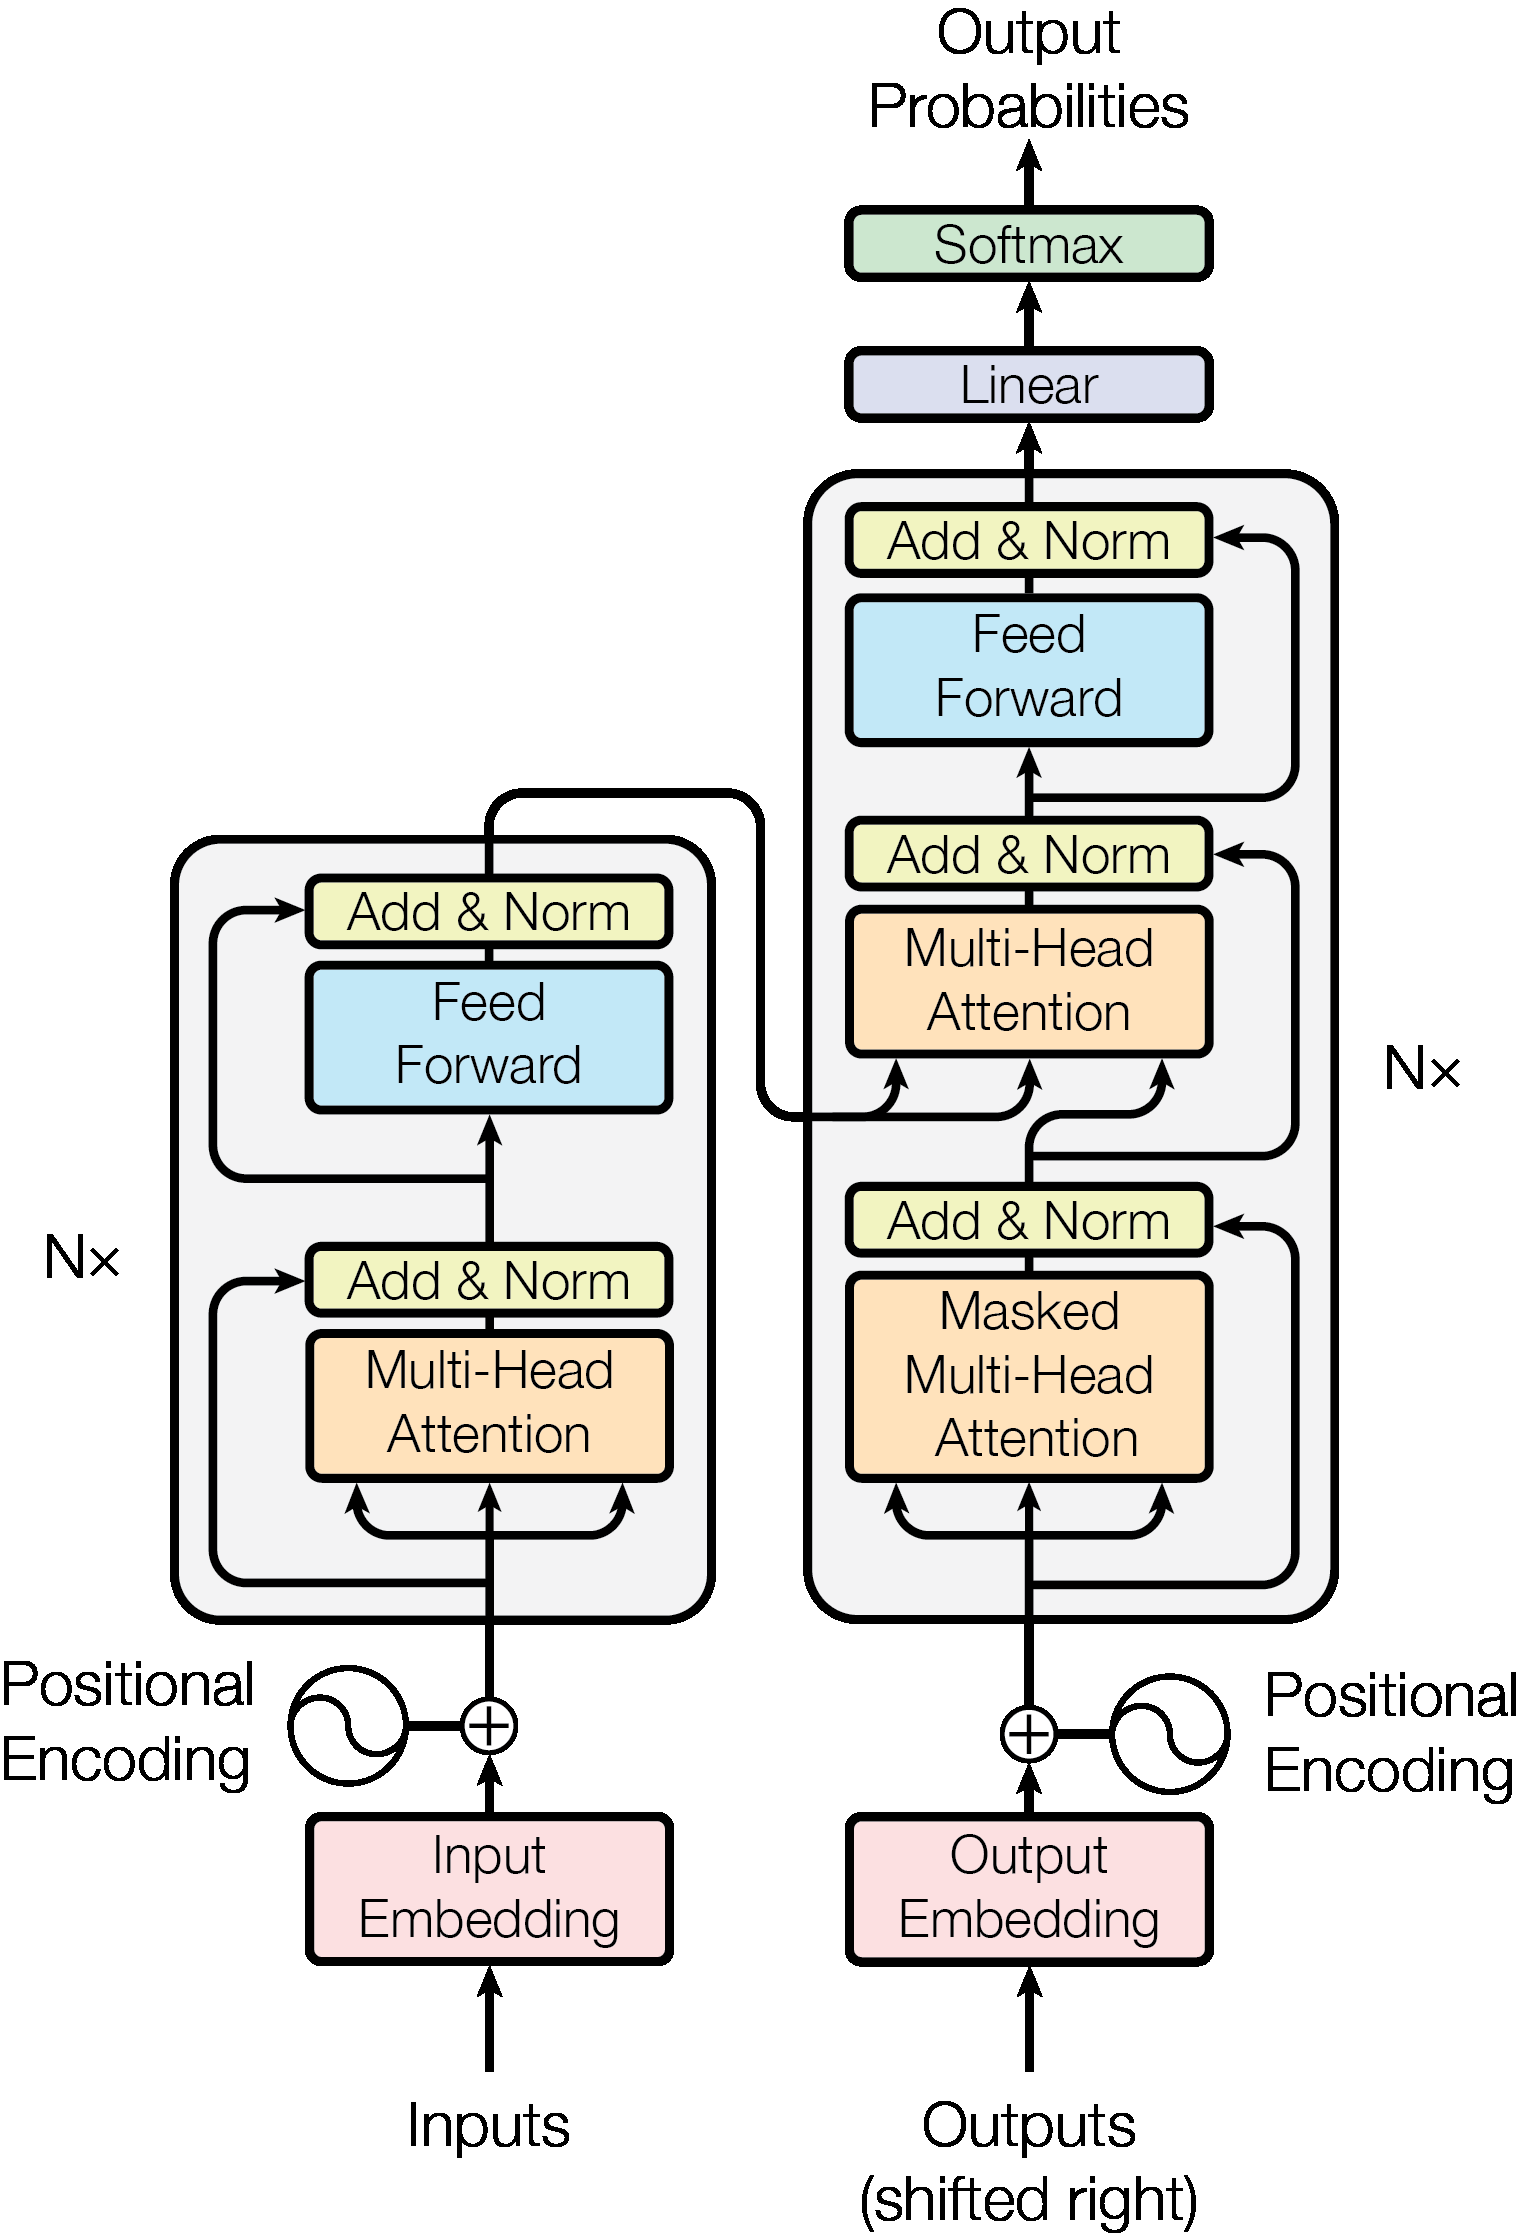
\includegraphics[width=\textwidth]{1}
		\column{.3\textwidth}
		\centering
		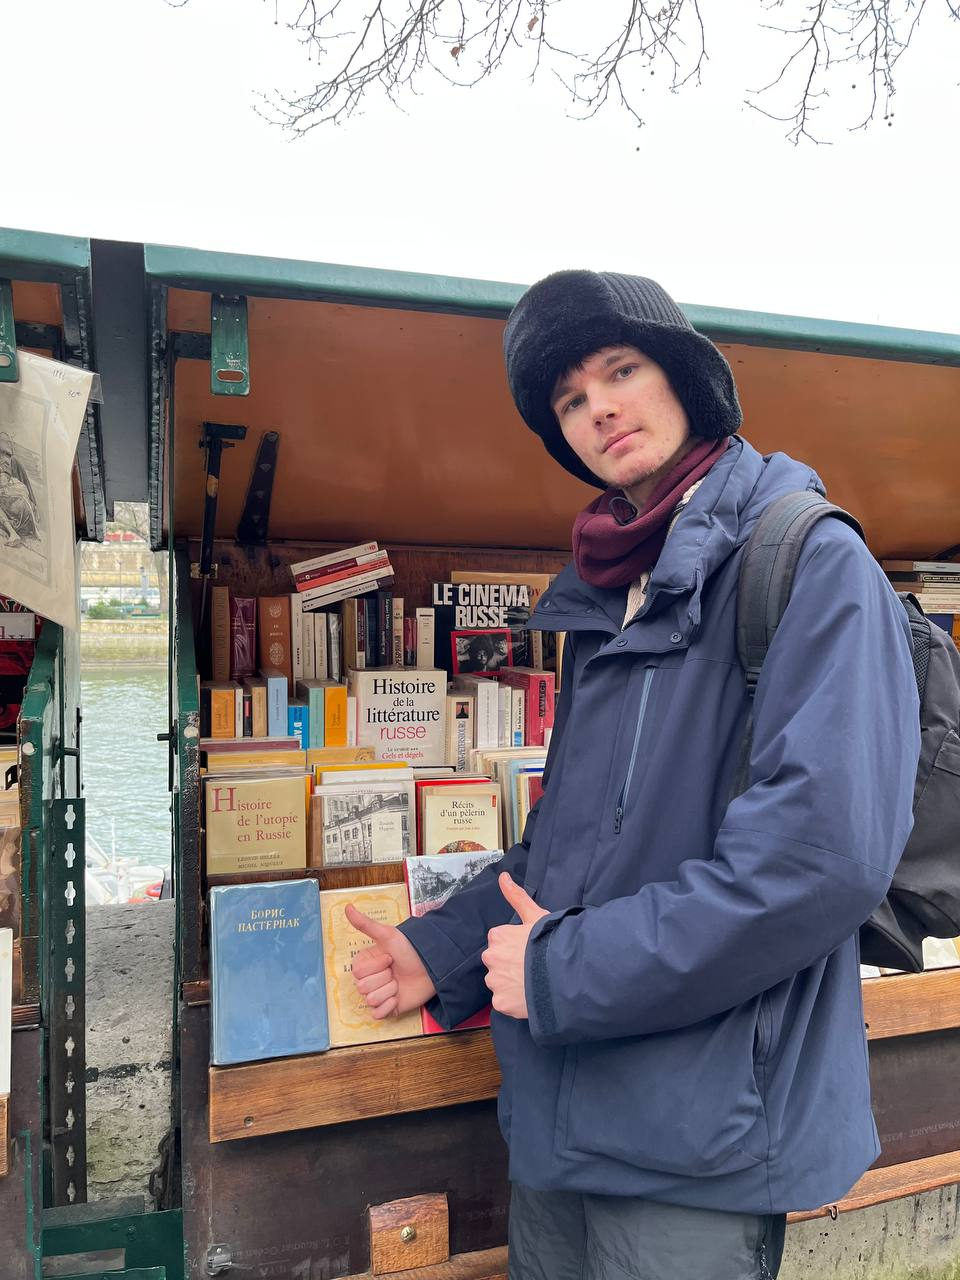
\includegraphics[width=\textwidth]{2}
		\column{.3\textwidth}
		\centering
		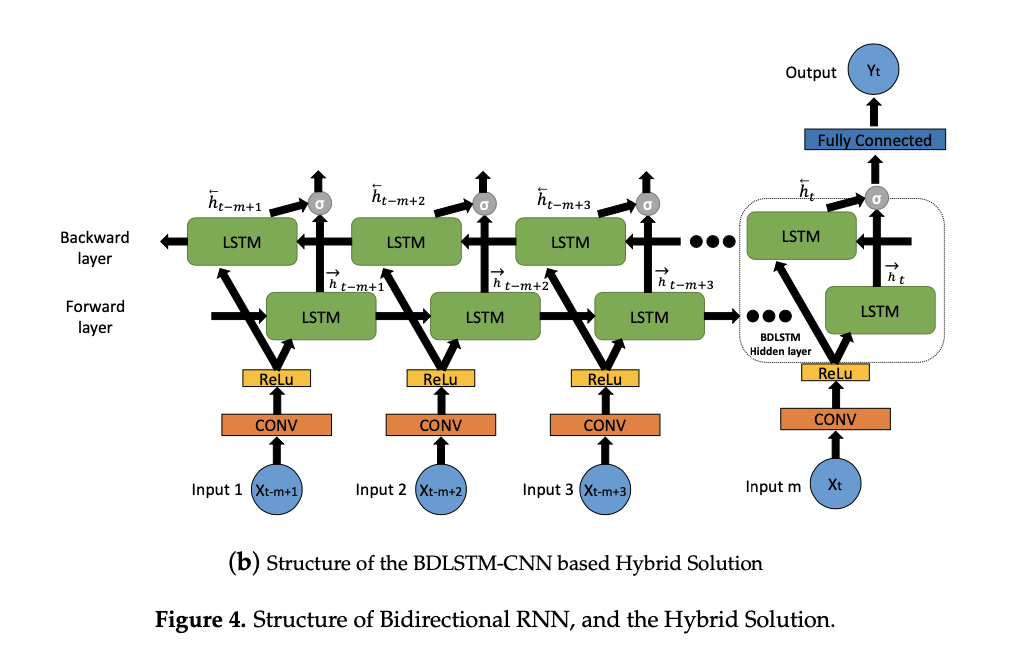
\includegraphics[width=\textwidth]{3}
	\end{columns}

\end{frame}

%\begin{frame}
%	\frametitle{Analyse de données et intelligence artificielle}
%	\begin{itemize}
%		\item ...
%		\item Analyse sensorielle
%		\item Optimisation des opérations viticoles
%		\item Peut-être tout?
%	\end{itemize}
%	
%	\begin{columns}[c]
%		\column{.7\textwidth}
%		\centering
%		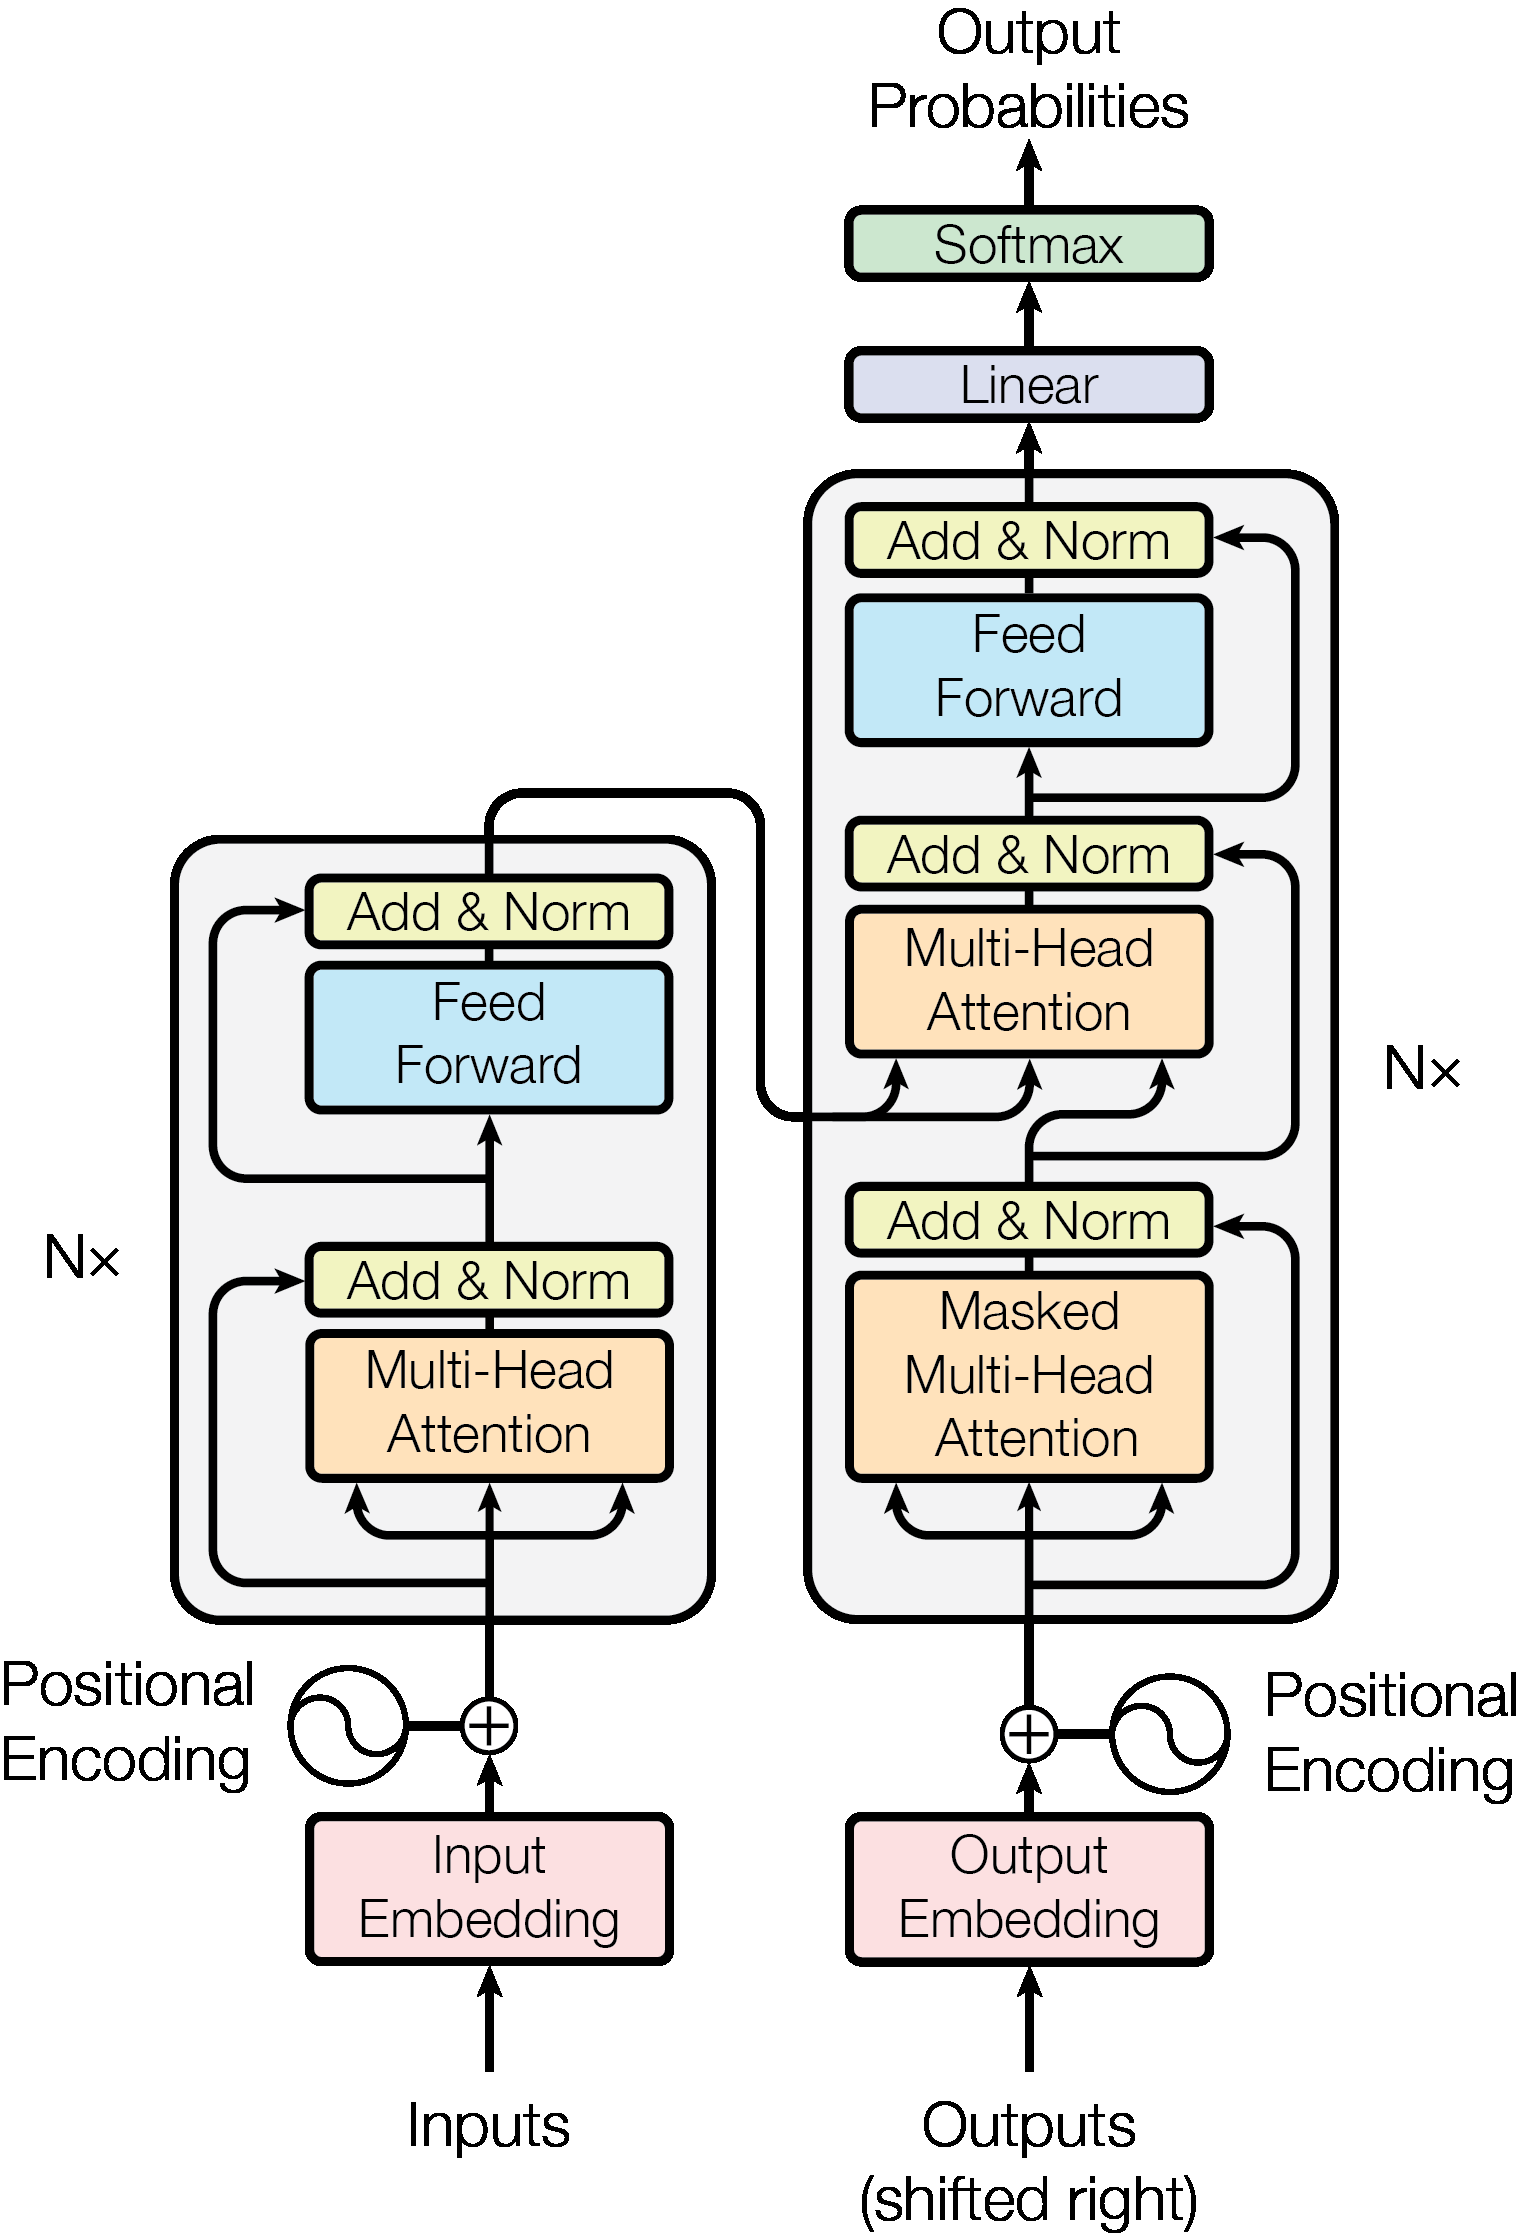
\includegraphics[width=\textwidth]{transformer}
%		\column{.2\textwidth}
%		\centering
%		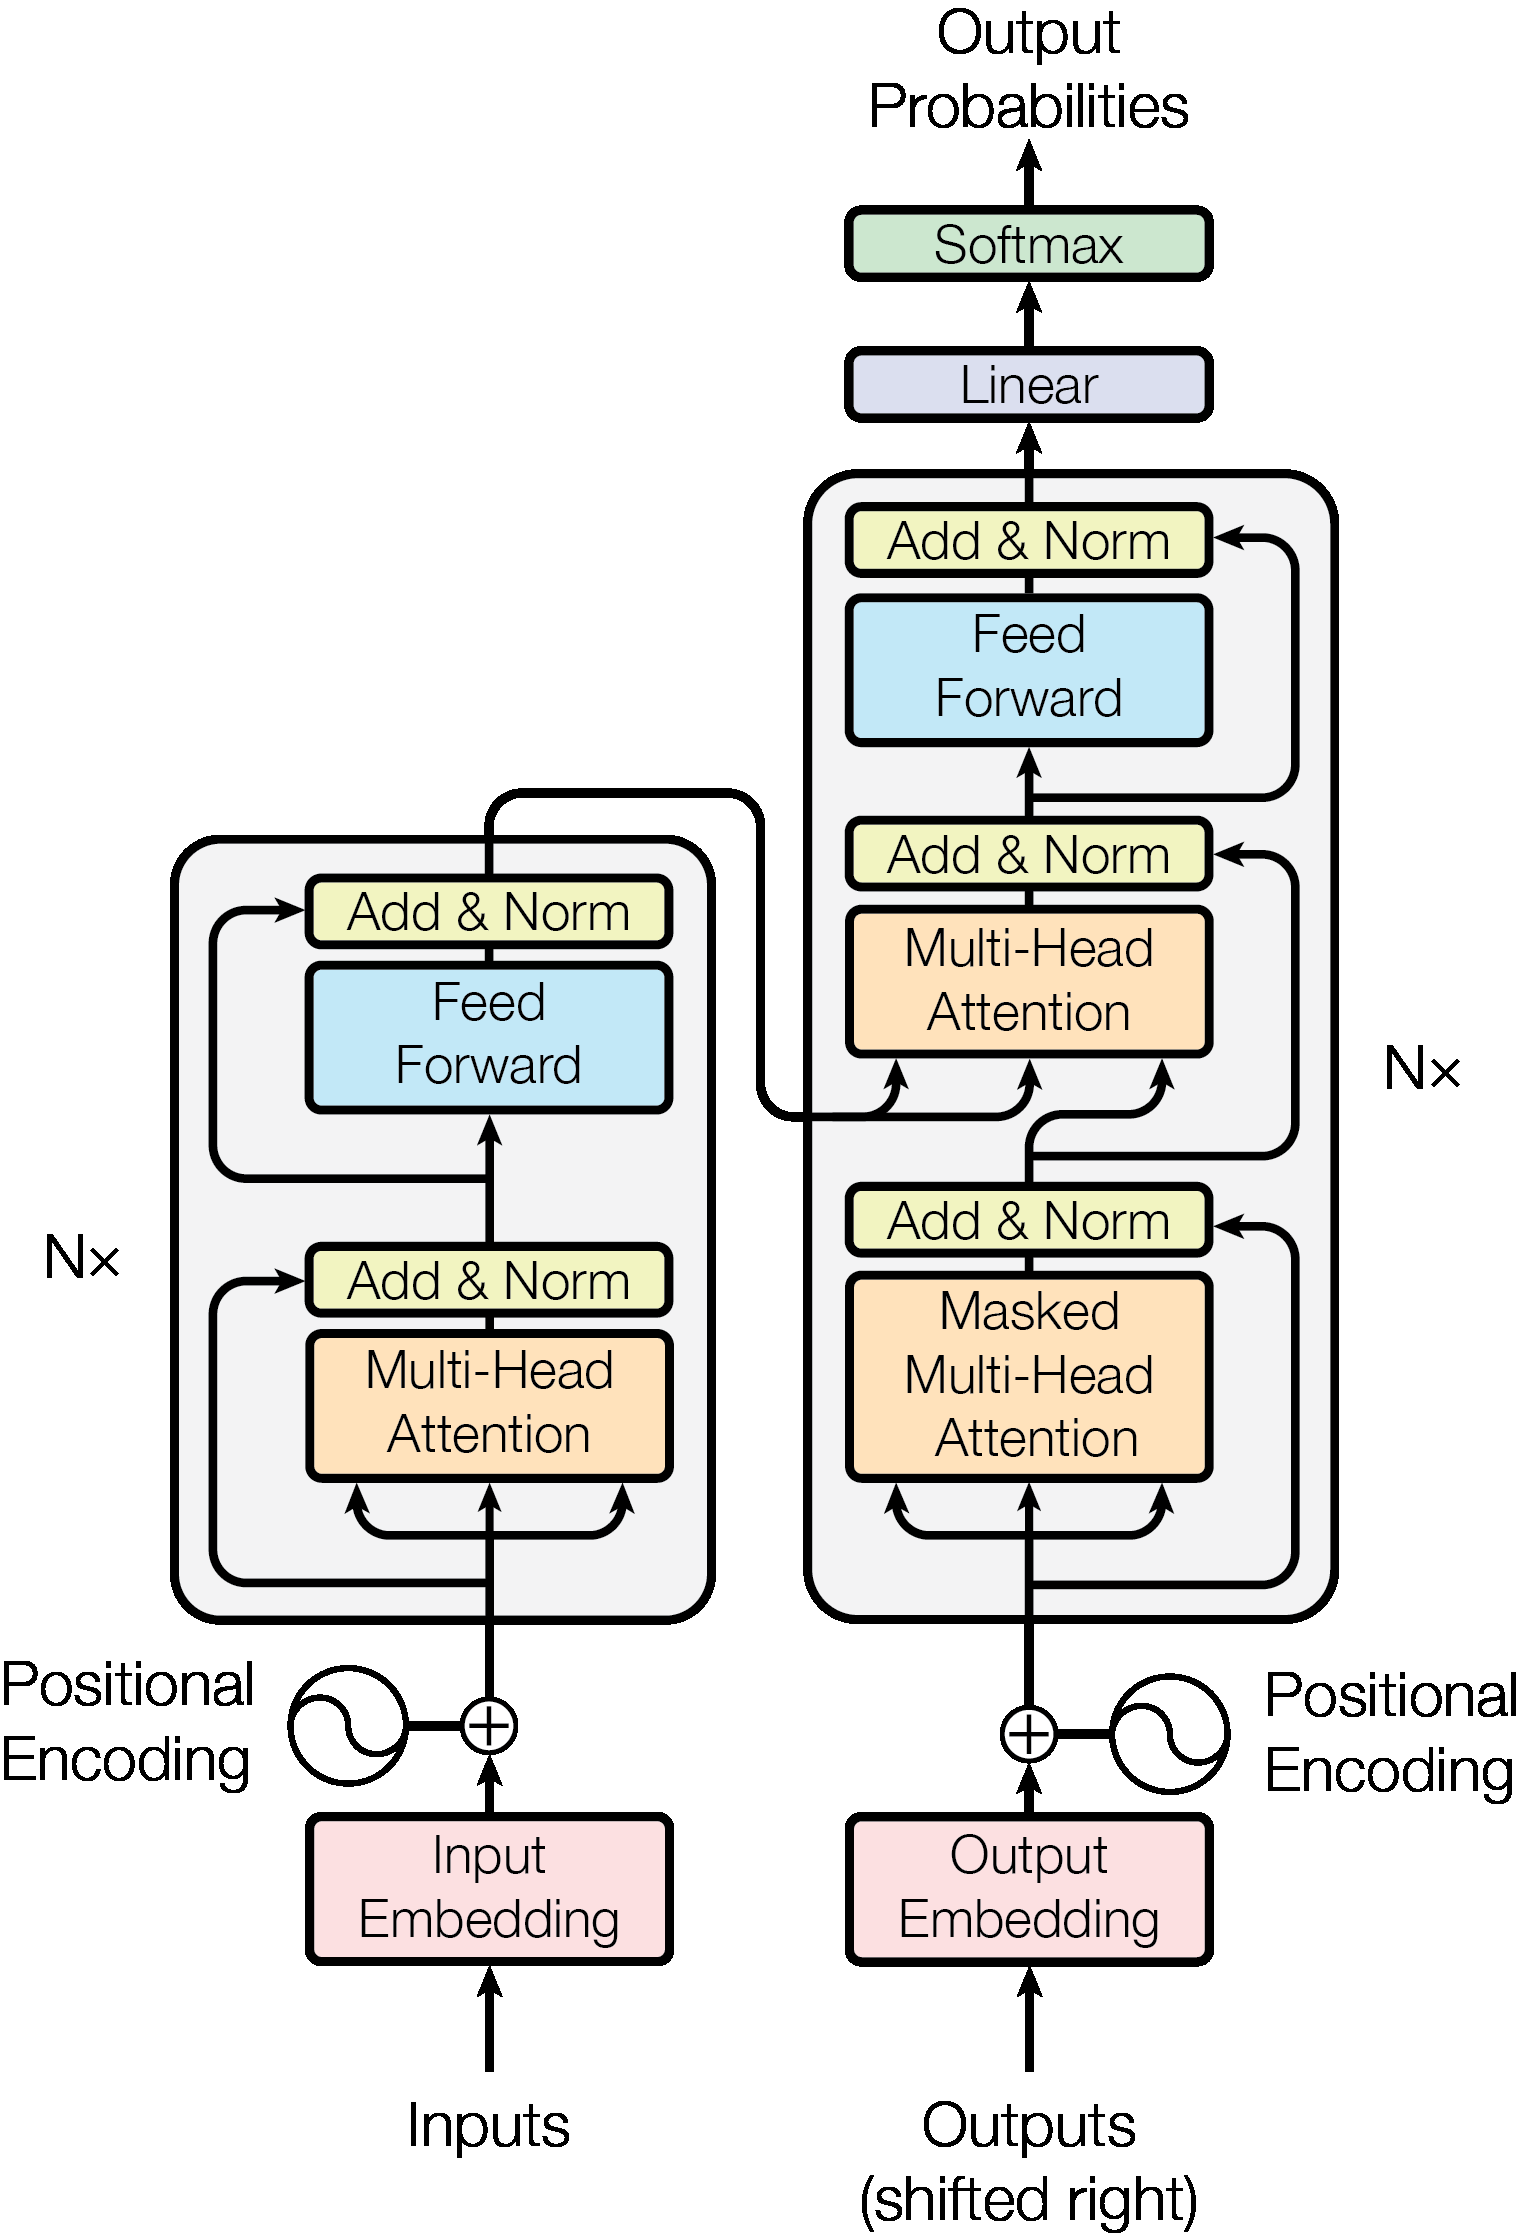
\includegraphics[width=\textwidth]{1}
%	\end{columns}
%	
%\end{frame}
\subsection{La revue et une analyse de l’état de l’art}

\begin{frame}
	\frametitle{La revue et une analyse de l’état de l’art}
	\begin{itemize}
		\item Le premier modèle TGN a apparu en 2020
		\item Les modèles TGN pour la modélisation portuaire régionale encore apparaissent
	\end{itemize}

	\begin{figure}
	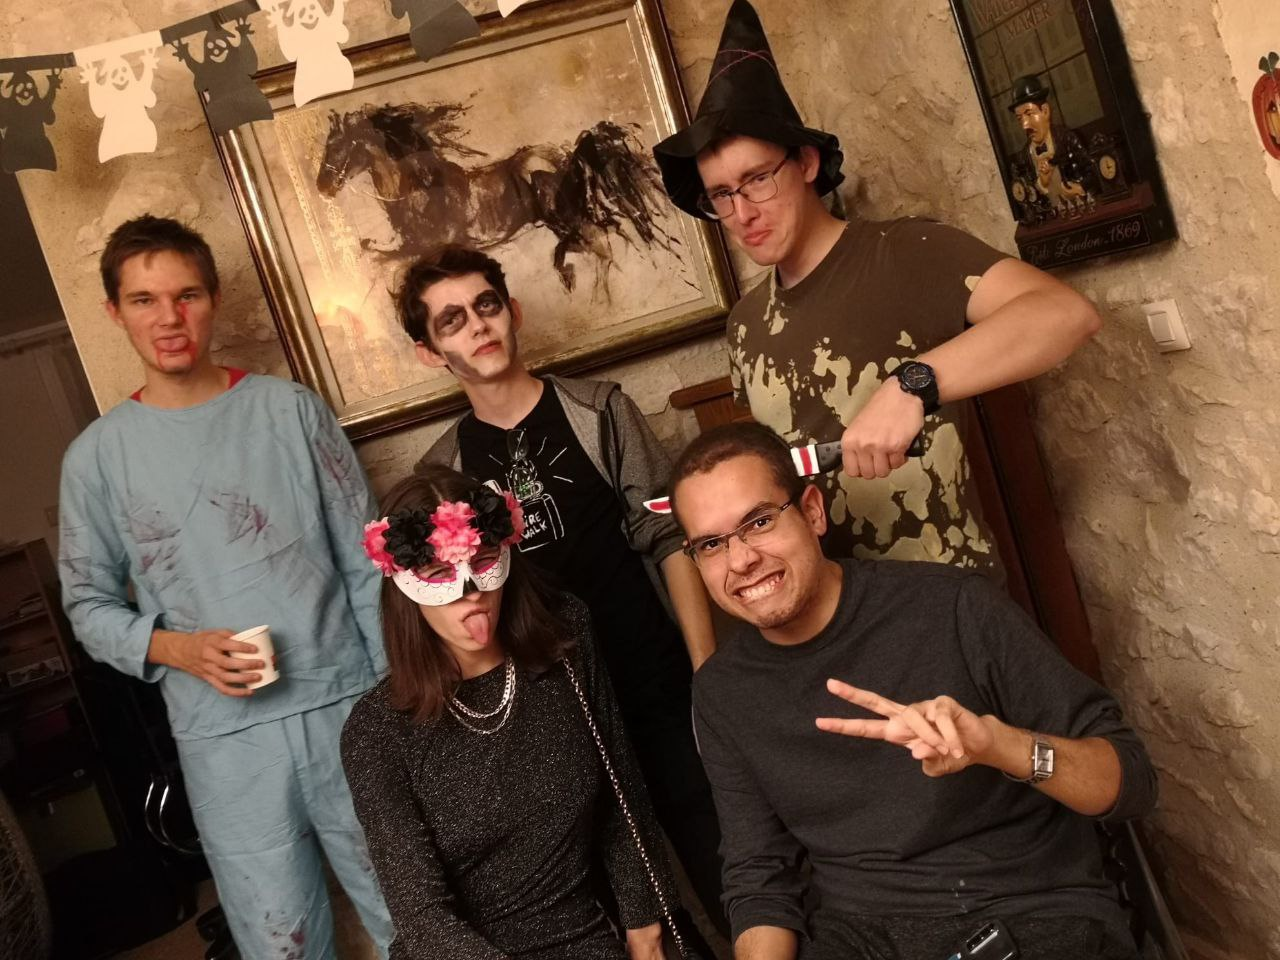
\includegraphics[width=0.8\textwidth]{4}
	\label{fig:example}
\end{figure}
	
\end{frame}

\begin{frame}
	\frametitle{Les avantages de TGN}
	Les avantages
	\begin{itemize}
		\item Modèle flexible par rapport aux caractérisations non-spatiales
		\item Modèle flexible par rapport aux caractérisations spatiales non-Euclidiens
		\item Modèle final et autonome
	\end{itemize}
	Les inconvénients 
	\begin{itemize}
		\item la nouveauté 
	\end{itemize}
	
	
\end{frame}


\section{Les objectifs intermédiaires et leur échéancier}

\begin{frame}
	\frametitle{Les objectifs intermédiaires et leur échéancier}
	\begin{enumerate}
		\item Les études de l'architecture, des frameworks utilisés – \textbf{Octobre 2023-Novembre 2023  }
		\item Les techniques courantes de l'apprentissage du GNN (state-of-art)– \textbf{Novembre 2023-Décembre 2023}
		\item Les brouillons de l'architecture du TGN pour nos tâches (type d'architecture) – \textbf{Décembre 2023-Janvier 2024}
		\item Réglage (embedding, couches) et retour au 3ème point – \textbf{Décembre 2023-Juin 2024}
	\end{enumerate}
\end{frame}

\section{L’organisation du travail et la répartition du travail}

		\begin{frame}
		\frametitle{L’organisation du travail et la répartition du travail}
		\begin{itemize}
			\item Isai – choix/réalisation de l'architecture, (choix de) traitement de données
			\item Borel – réalisation de l'architecture, traitement de données
			\item Ruflin – réalisation de l'architecture, traitement de données
			\item Merciel – réalisation de l'architecture, traitement de données
		\end{itemize}
	
	
	\end{frame}

\section{L’identification des moyens auxquels le projet fera appel}

		\begin{frame}
	\frametitle{L’organisation du travail et la répartition du travail}
	Le projet est soutenu entièrement par CMA CGM
	\begin{itemize}
		\item Données
		\item GPU
		\item Platforme de stockage et d'exécution 
		\item Consultations et retour
	\end{itemize}
	
	
\end{frame}
	

	\begin{frame}
	\begin{center}
{\LARGE Merci pour votre attention }
	\end{center}
\end{frame}



	
\end{document}
